\documentclass[a4paper,12pt]{report}

\usepackage[brazilian,english]{babel}
\usepackage{indentfirst}
\usepackage{a4wide}
\usepackage[section]{placeins}
\usepackage[utf8]{inputenc}
% \usepackage[Conny]{fncychap}
\usepackage[T1]{fontenc}
\usepackage{txfonts}
\usepackage{type1cm}
\usepackage{courier}
\usepackage[scaled]{helvet}
\usepackage{epigraph}
\renewcommand*\familydefault{\sfdefault}

\hyphenation{
  es-ta-be-le-ci-do
  a-de-qua-da-men-te
  pro-ble-mas
  di-men-sio-na-men-to
  mo-de-lo
}

% Controlar linhas orfas e viuvas
\clubpenalty=10000
\widowpenalty=10000
\displaywidowpenalty=10000

% Formatar notas de rodape
\usepackage[hang]{footmisc}
\setlength{\footnotemargin}{1em}

\usepackage{url}
%% Define a new 'leo' style for the package that will use a smaller font.
\makeatletter
\def\url@leostyle{%
  \@ifundefined{selectfont}{\def\UrlFont{\sf}}{\def\UrlFont{\small\ttfamily}}}
\makeatother
%% Now actually use the newly defined style.
\urlstyle{leo}

\usepackage[left=3cm,top=3cm,right=2cm,bottom=2cm,includehead,ignoremp]{geometry}

\usepackage[small]{titlesec}
% \titlespacing{\chapter}{0pt}{-50pt}{*20}[0pt]
\titlespacing{\chapter}{0pt}{*-10}{*5}

% Running Headers and footers
\usepackage{fancyhdr}
% \pagestyle{fancy}
\pagestyle{headings}
% Redefine plain page style
\fancypagestyle{plain}{
  \fancyhf{}
  \renewcommand{\headrulewidth}{0pt}
  \fancyhead[LE,RO]{\thepage}
}

\linespread{1.3}
%\pdfpagewidth=\paperwidth
%\pdfpageheight=\paperheight

% Para habilitar cálculos em dimensões
\usepackage{calc}

% Multipart figures
%\usepackage{subfigure}

% More symbols
%\usepackage{amsmath}
%\usepackage{amssymb}
%\usepackage{latexsym}

% Surround parts of graphics with box
\usepackage{boxedminipage}

% Package for including code in the document
\usepackage{listings}

% If you want to generate a toc for each chapter (use with book)
%\usepackage{minitoc}

% This is now the recommended way for checking for PDFLaTeX:
\usepackage{ifpdf}

\ifpdf
\usepackage[pdftex]{graphicx}
\else
\usepackage{graphicx}
\fi

\title{Dionisio}
\author{Allan Douglas R. de Oliveira \\ allandouglas@gmail.com \and
Leonardo Nicacio Bessa \\ leobessa@gmail.com \and
Thiago Rodrigues Andrade \\ suffragium@gmail.com}
\date{2009-04-22}

\usepackage[absolute]{textpos}
\begin{document}

\ifpdf
\DeclareGraphicsExtensions{.png, .pdf, .jpg, .tif}
\else
\DeclareGraphicsExtensions{.eps, .jpg}
\fi

%\maketitle
\pagestyle{empty}
\begin{center}
  {\large ALLAN DOUGLAS R. DE OLIVEIRA \\
    LEONARDO NICACIO BESSA \\
    THIAGO RODRIGUES ANDRADE}
\end{center}

\begin{textblock*}{21cm}[0,0](0cm,12cm)
  \begin{center}
    {\LARGE Dionisio:\\ Um sistema de recomendação baseado em confiança }
  \end{center}
\end{textblock*}


\begin{textblock*}{21cm}[0,0](0cm,29.7cm-4cm)
  \begin{center}
    {\large São Paulo \\ 2009 }
  \end{center}
\end{textblock*}

\newpage
\begin{center}
  {\large ALLAN DOUGLAS R. DE OLIVEIRA \\
    LEONARDO NICACIO BESSA \\
    THIAGO RODRIGUES ANDRADE}
\end{center}

\begin{textblock*}{21cm}[0,0](0cm,12cm)
  \begin{center}
    {\LARGE Dionisio:\\ Um sistema de recomendação baseado em confiança }
  \end{center}
\end{textblock*}


\begin{textblock*}{21cm}[0,0](0cm,29.7cm-4cm)
  \begin{center}
    {\large São Paulo \\ 2009 }
  \end{center}
\end{textblock*}


\begin{textblock*}{21cm/2-2cm}[0,0](21cm/2,15cm)
  \begin{flushleft}
    {\large
  Monografia apresentada à Escola Politécnica da Universidade de São Paulo para obtenção do título de Bacharel em Engenharia.\newline
  \newline
  Área de Concentração:\newline
  Engenharia de Computação\newline
}
  \end{flushleft}
\end{textblock*}



\begin{center}
  {\large ALLAN DOUGLAS R. DE OLIVEIRA \\
    LEONARDO NICACIO BESSA \\
    THIAGO RODRIGUES ANDRADE}
\end{center}

\begin{textblock*}{21cm}[0,0](0cm,12cm)
  \begin{center}
    {\LARGE Dionisio:\\ Um sistema de recomendação baseado em confiança }
  \end{center}
\end{textblock*}


\begin{textblock*}{21cm}[0,0](0cm,29.7cm-4cm)
  \begin{center}
    {\large São Paulo \\ 2009 }
  \end{center}
\end{textblock*}


\begin{textblock*}{21cm/2-2cm}[0,0](21cm/2,15cm)
  \begin{flushleft}
    {\large
  Monografia apresentada à Escola Politécnica da Universidade de São Paulo para obtenção do título de Bacharel em Engenharia.\newline
  \newline
  Área de Concentração:\newline
  Engenharia de Computação\newline
}

    {\large
      Orientador: Prof. Dr. Jaime Simão Sichman \\
        Co-orientadora: Prof. Dra. Lucia Filgueiras
    }
  \end{flushleft}
\end{textblock*}


%\begin{textblock*}{21cm/3}[0,0](21cm/3*2-2cm,29.7cm-6cm)
  \begin{flushright}
    {\emph{
           Aos nossos pais e companheiras, pelo apoio e incentivo em nossa formação pessoal. Aos mestres, pelo conhecimento transmitido e pela paciência que tiveram conosco.
          }
    }
  \end{flushright}
\end{textblock*}

\null\newpage


% agradecimentos (opcional)
%\begin{textblock*}{21cm/3}[0,0](21cm/3*2-2cm,29.7cm-6cm)
  \begin{flushright}
\epigraph{\emph{``Innovation distinguishes between a leader and a follower.''}}{Steven Paul Jobs\\Co-fundador da Apple Inc.}
\end{flushright}
\end{textblock*}

\null\newpage


\pagenumbering{roman}

% Resumo e Abstract
\selectlanguage{brazilian}
%  \begin{abstract}
%    O comércio eletrônico brasileiro tem evoluído em termos de serviços prestados ao consumidor. Este trabalho apresenta a especificação e implementação de um sistema online de recomendação para facilitar o encontro do usuário com os produtos e serviços mais relevantes a ele. Para isso, são descritos em detalhes os requisitos funcionais e não funcionais do sistema, os algoritmos de recomendação utilizados e as escolhas na implementação do projeto. 
O sistema projetado é composto por três algoritmos de recomendação, sendo dois deles já difundidos, enquanto o terceiro é um novo, e que foi proposto para levar em consideração as relações de confiança do usuário com seus pares. 
A execução deste trabalho incluiu a realização de um experimento com pessoas interagindo com o sistema de recomendação através de uma rede social. A análise do experimento é apresentada através de gráficos e dados estatísticos que comparam os algoritmos utilizados. 
Os resultados do projeto podem ser aplicados no futuro no desenvolvimento de lojas virtuais online e/ou aplicativos de redes sociais.
%  \end{abstract}
%\begin{otherlanguage}{english}
%  \begin{abstract}
%    The Brazilian e-commerce has evolved in terms of services provided to the consumer. This paper presents the specification and implementation of an online recommendation system that eases the matching of a user with the most relevant products and services. Furthermore the functional and non-functional system requirements, the selected recommendation algorithms and the choices made in the implementation are described in detail.
The designed system consists of three recommendation algorithms, two of them are already widely spreaded, while the third one is new and was proposed to consider the trust among users and their peers.
This work also includes an experiment with people interacting with the recommendation system through a social network. The analysis of the experiment is presented through graphs and statistics that compare the algorithms.
The results of the project can be applied in future development of virtual online stores and/or social networking applications.
%  \end{abstract}
%\end{otherlanguage}

%\listoffigures \thispagestyle{headings} % Lista de Figuras

% \listoftables \thispagestyle{empty} % Lista de Tabelas

\tableofcontents \thispagestyle{headings} % Sumario

% lista de abreviaturas e siglas (opcional)
% lista de simbolos (opcional)

\pagestyle{headings}

% Elementos de Texto
\chapter{INTRODUÇÃO} \pagenumbering{arabic} % (fold)

\section{Objetivo} % (fold)
\label{sec:objetivo}
% Apresentar de forma precisa e concisa o objetivo do projeto.

 O principal objetivo deste projeto é criar um sistema de recomendação baseado em recursos disponíveis na Web, que possibilite a sugestão de itens confiáveis e relevantes ao usuário.

% section objetivo (end)

\section{Motivação} % (fold)
\label{sec:motivação}

% O que é importante para: nós, comunidade científica, usuários, mercado.

% Apresentar a motivação e justificativa para a realização do trabalho (por exemplo, sua aplicabilidade prática, comparação com alternativas já existentes, potencial de  aprendizado e evolução, etc).

% http://www.uxmatters.com/mt/archives/2009/03/including-recommendations-in-user-interfaces-to-enhance-motivation.phps

 Sistemas de Recomendação sugerem aos usuários itens que eles possam gostar, baseado no comportamento prévio do usuário. Fazendo suposições pertinentes sobre o tipo de objetos em que os usuários estão interessados, é possível conquistar a sua confiança. A vantagem para os usuários é a facilidade de encontrar a informação, sem ter a árdua tarefa de procurá-la.

 As redes sociais online têm modificado a forma com que as empresas utilizam a comunicação para o comércio. Pessoas estão utilizando a Web para encontrar outras pessoas com interesses similares, fazer compras de forma mais eficiente, aprender sobre produtos e serviços e reclamar sobre produtos malfeitos\cite{marketing_social_web}.

 A Web está rapidamente se tornando a mídia mais importante para o marketing. A tendência é que as pessoas cada vez mais bloqueiem os anúncios indesejados e queiram ter a capacidade de encontrar os produtos relevantes no momento adequado. É nesse contexto que surge a necessidade de uma plataforma que facilite a colaboração e que permita a criação e classificação de conteúdo pelos consumidores, de forma a permitir uma escolha mais inteligente dos melhores produtos e serviços, e ao mesmo tempo criando uma mecanismo de feedback para as empresas interessadas.

 Devido à grande variedade atual de produtos e serviços, as pessoas têm cada vez mais dificuldade nas suas escolhas e na argumentação sobre a possível decisão. Quanto maior for a quantidade de produtos similares de fabricantes diferentes, mais as pessoas se vêem desnorteadas e sem saber se a decisão realizada foi a mais correta.
 
 % TODO: Escrever sobre Web Semântica

% paragraph paragraph_name (end)
% section motivação (end)

%\section{Organização} % (fold)
%\label{sec:organização}

% Não fazer ainda!!!
% Apresentar a organização do documento: o que cada capítulo, anexo e apêndice aborda.


% section organização (end)

% chapter web_social (end)
\chapter{SISTEMAS DE RECOMENDAÇÃO} \pagenumbering{arabic}% (fold)
\label{cha:sistemas_de_recomendação}

\section{Introdução}
Sistemas de recomendação~\footnote{Em inglês, \textit{Recommender systems}.} são aqueles que sugerem itens ao seus usuários de forma a ajudá-los a encontrar mais efetivamente os itens de maior interesse dentre uma variedade imensa de opções.

A idéia de recomendar itens é algo que pode ser observado no dia-a-dia das pessoas. Como muitas escolhas precisam ser feitas sem que se tenha uma experiência pessoal das alternativas, as pessoas se baseiam no que as outras dizem sobre um determinado produto antes de comprá-lo ou experimentá-lo. Estas informações são transmitidas boca-a-boca entre amigos e colegas ou através de resenhas especializadas que podem encontradas em revistas e jornais.

Os sistemas de recomendação auxiliam este processo social, agregando opiniões e avaliações de uma comunidade de usuários sobre os produtos e recomendando itens de acordo com o perfil do usuário desta comunidade.

\section{Contexto histórico}
O primeiro sistema de recomendação, Tapestry~\footnote{Ver \cite{Goldberg92}.}, foi desenvolvido no início da década de 90.~\cite{Resnick97} Na última década o sistemas, principalmente os baseado em filtragem colaborativa, foram um grande foco de estudo~\cite{Herlocker04}.

Graças ao acumulo de informações provenientes da web social, observa-se hoje que vários sistemas de recomendação podem ser experimentados pelo usuários da Internet, como exemplo:

\begin{itemize}
\item 
A Amazon~\footnote{http://www.amazon.com} e o Submarino~\footnote{http://www.submarino.com.br.}, lojas virtuais de artigos diversos, recomendam itens semelhantes para aqueles usuários que compram um produto ou manifestam interesse em comprá-lo.

\item O Last.fm~\footnote{http://last.fm.}, uma rede social focada em música, recomenda artistas e canções semelhantes àquelas que os usuários mais gostam de ouvir.

\item O Digg~\footnote{http://digg.com.} e o Delicious~\footnote{http://del.icio.us.}, sistemas de compartilhamento de links~\footnote{Também conhecidos como bookmarks.}, geram uma lista geral de links recomendados baseado nas opiniões dos usuários do sistema.

\item O StumbleUpon~\footnote{http://stumbleupon.com.}, também um sistema online de compartilhamento de links, permite que os usuários recebam recomendações de links e avaliem se eles gostaram ou não daquele link, gerando recomendações personalizadas baseadas nessa avaliação.
\end{itemize}


\section{Classificações dos sistemas de recomendação}

Nas próximas seções serão apresentadas as diferentes abordagens para a implementação de sistemas de recomendação. As primeiras abordagens foram a filtragem colaborativa e a filtragem baseada em conteúdo. Vários sistemas são híbridos, isto é, utilizam mais de uma abordagem.

%Na seção (seção XXX) serão discutidos as diferentes implementações encontradas na literatura.

\section{Filtragem baseada em conteúdo} % (fold)
A filtragem baseada em conteúdo consiste na extração de \textit{features} dos itens a serem recomendados e da comparação desses \textit{features} com aqueles que formam o  perfil histórico do usuário. Esse é um dos primeiros métodos que surgiram e sua origem está na comunidade de \textit{information retrieval}.~\cite{Balabanovi97}

Como exemplo, suponha-se que se queira recomendar documentos em formato texto. Os \textit{features} nesse caso poderiam ser as palavras do texto. O perfil histórico do usuário seria formado pela frequência acumulada das palavras presentes em cada texto avaliado pelo usuário. Um documento neste caso é recomendado se os \textit{features} (palavras) presentes podem ser encontrados em grande frequência nos documentos avaliados positivamente pelo usuário no passado.

Outros exemplos de \textit{features} que podem ser usados em um documento são meta-informações como autor, categoria do documento (artigo, jornal, revista, por exemplo), assunto (computação, matemática, artes, esportes), entre outras palavras-chave.

% (falar um pouquinho porque é bom/ruim)

\section{Filtragem social} % (fold)

% Talvez usar o Pazzani96syskill para falar de content-based

A filtragem social\footnote{Termo originado em \cite{Malone87} segundo \cite{Hill95}.} consiste em um conjunto de técnicas que utilizam o contexto e as relações sociais de uma comunidade de usuários para fazer recomendações. Ao contrário da filtragem colaborativa, o conteúdo de cada item não é analisado, possibilitando-se recomendar qualquer tipo de item.

\subsection{Filtragem colaborativa}

O termo \textit{collaborative filtering} foi cunhado por \cite{Goldberg92}~\footnote{Conforme \cite{Resnick97}.}. A abordagem básica consiste em montar um sistema que permite os usuários fazerem avaliações\footnote{Em inglês, \textit{ratings} ou \textit{votes}.} dos itens que podem ser recomendados. Isso resulta em triplas (usuário, item, avaliação). A partir dessas avaliações, pode-se criar uma lista de recomendação para um determinado usuário. Na descrição a seguir, este usuário a quem se deseja recomendar algo será chamado usuário ativo. A avaliação de um item feita por um usuário será chamada de voto. Os passos são os seguintes:

\begin{enumerate}
\item 
Para cada usuário do sistema, determina-se a similaridade entre este usuário e o usuário ativo. Este valor será designado por $s$.

\item Para cada item do sistema não avaliado pelo usuário ativo, calcula-se o voto previsto $p$ para aquele item utilizando-se o voto de cada usuário que avaliou o item e a similaridade $s$ entre o usuário e o usuário ativo. O voto previsto é uma estimativa da avaliação que aquele usuário faria do item caso já o conhecesse.
\end{enumerate}

\paragraph{Geração de uma lista de recomendação de tamanho $n$.}

A lista de itens recomendados será formada pelos $n$ itens com os maiores votos previstos ordenados decrescentemente.

\subsubsection{Formulação matemática}
Mais detalhadamente, o algoritmo básico é o seguinte:

Sendo $v_{i,j}$ o voto do usuário $i$ para o item $j$, $I_{i}$ o conjunto de itens que foram avaliados pelo usuário $i$, define-se voto médio de um usuário $i$ por:

\begin{equation}
 \bar{v_{i}} = \frac{1}{|I_{i}|} \sum_{j \in I_{i}} v_{i,j}
\end{equation}

O valor previsto do voto do usuário ativo $a$ para o item $j$, será dado por:

\begin{equation}
 p_{a,j} = \bar{v_{a}} + k\sum_{i=1}^n{s(a,i) (v_{i,j} - \bar{v_{i})}}
 \label{eq:filtragem_colaborativa_similaridade} 
\end{equation}
onde $n$ é o número de usuários do sistema, $s(a,i)$ é a similaridade entre o usuário $a$ e o usuário $i$ e $k$ é um fator de normalização, dado neste caso por:

\begin{equation}
 k = \sum_{i=1}^n{\frac{1}{s(a,i)}}
\end{equation}


\paragraph{Cálculo de $s$.}

O cálculo de $s$ geralmente é realizado utilizando-se o coeficiente de correlação de Pearson\cite{Breese98}, definido por:

\begin{equation}
 s(a,i) = \frac{\sum_{j}{(v_{a,j} - \bar{v_{a}}) (v_{i,j} - \bar{v_{i}})}}{\sqrt{\sum_{j}{(v_{a,j} - \bar{v_{a}})}^2\sum_{j}{(v_{i,j} - \bar{v_{i}})}^2}}
\end{equation}

\paragraph{Forma geral da Filtragem Colaborativa.}

Apesar dos primeiras abordagens terem utilizado a similaridade $s$, qualquer peso $w$\footnote{Do inglês \textit{weigth}} pode ser usado na equação \ref{eq:filtragem_colaborativa_similaridade}. Pode-se então reescreve-la da seguinte maneira geral:

\begin{equation}
 p_{a,j} = \bar{v_{a}} + k\sum_{i=1}^n{w(a,i) (v_{i,j} - \bar{v_{i})}}
 \label{eq:filtragem_colaborativa_geral} 
\end{equation}

Para mais detalhes, ver \cite{Breese98}.
% Explicar com mais detalhes o método e citar outros tipos de w


\subsection{Filtragem baseada em confiança} % (fold)

A filtragem baseada em confiança\footnote{Entendida aqui no contexto de \textit{Trust-aware recommender systems}~\cite{Massa07}} é muito similar à filtragem colaborativa, mas utiliza como peso $w(a,i)$ a confiança do usuário $a$ no usuário $i$.

Esta confiança é fornecida de forma explícita pelo usuário. Este método se mostrou muito efetivo no casos em que a maioria dos usuários do sistema são \textit{cold-users}, isto é, quando a maioria dos usuários avaliou poucos itens e portanto possuem poucos itens em comum. Em um cenário como esse a filtragem colaborativa tradicional falha em encontrar usuários semelhantes pois há pouca intersecção de avaliações de itens~\footnote{Em inglês, \textit{rating-overlap}.}.

%\section{

%\section{Discussão sobre as diferentes abordagens}



\chapter{WEB SOCIAL} % (fold)
\label{cha:web_social}

% Qual é a melhor solução neste contexto?

% Por que ela depende de recomendação?

% chapter web_social (end)
\chapter{WEB SEMÂNTICA} % (fold)
\label{cha:web_semantica}
% Tecnologias e conceitos empregados, contextualização do Projeto de Formatura em sua área de aplicação, revisão da literatura.

\section{World Wide Web} % (fold)
\label{sec:world_wide_web}

A World Wide Web é um sistema de documentos em hipermídia que são interligados e executados na Internet. A maioria do conteúdo disponível na Web atualmente é projetado para a leitura por seres humanos. A utilização de programas de computador para interpretação desse conteúdo é complexa devido à baixa flexibilidade dos programas em relação aos humanos. Se por um lado os aplicativos são menos flexíveis que os seres humanos para interpretação de textos, por outro eles são capazes de desenvolver e analisar estruturas de dados complexas. A Web Semântica, apresentada a seguir, baseia-se nessa virtude do software. 

% Novas tecnologias como RSS, XML-RPC e SOAP foram desenvolvidas para facilitar o acesso a algumas informações disponíveis nas páginas da Web.

Segundo Berners-Lee \cite{bemerslee2001sw}, a Web Semântica não é uma Web separada, mas um extensão da atual, na qual a informação é disponibilizada com sentido bem definido, aprimorando a capacidade de cooperação entre pessoas e computadores. Os documentos nesta extensão da Web são convenientes para utilização tanto por humanos como por programas.

% 2.	A WS precisará de uma base de dados centralizada para poder raciocinar?

Da mesma forma que os humanos buscam informações em bases de dados descentralizadas na Web, com a adoção da Web Semântica agentes computacionais poderão fazer o mesmo. Essa descentralização de documentos permite que inconsistências ocorram, porém possibilita um rápido crescimento no volume de dados.

%The Semantic Web is not a separate Web but an extension of the current one, in which information is given well-defined meaning, better enabling computers and people to work in cooperation.

A W3C realiza trabalhos para aprimorar, extender e padronizar a Web. Com o apoio de uma equipe especializada do consórcio, tecnologias para representação estrutural e semântica dos recursos na Web foram desenvoldidas, resultando em um conjunto de especificações para a Web Semântica. Atualmente este conjunto é basicamente composto pelo Resource Description Framework (RDF), a linguagem RDF Schema e a Web Ontology Language (OWL).

% TODO: [OWL]... melhor explicado nas seções seguintes. 

% 3.	Explicar a diferença entre apresentar dados e entender dados no contexto da web atual?

Os mecanismos de busca atualmente utilizados na Web são capazes de listar os sites que contenham os termos desejados, bem como orderná-los de acordo com critérios de relevância. Considerando as dificuldades impostas à interpretação do conteúdo pelos computadores, fica a cargo do usuário a tarefa de identificar quais dos sites obtidos são coerentes com as expectativas de contexto e necessidade.

% { Nessa direção, Souza e Alvarenga (2004) consideram que a dificuldade em determinar os contextos informacionais tem como conseqüência a impossibilidade de se identificar de forma precisa a atinência dos documentos. Além disso, a ênfase das tecnologias e linguagens utilizadas nas páginas da Web tradicional focaliza os aspectos de exibição e apresentação dos dados, de uma forma que a informação seja descrita pobremente e pouco passível de ser consumida concomitantemente por máquinas e seres humanos. A partir disso é que surge a proposta da Web Semântica.} [][http://www.scielo.br/scielo.php?pid=S1413-99362007000100006&script=sci_arttext| Web Semântica: ontologias como ferramentas de representação do conhecimento]]

%\subsection{Protocolo HTTP} % (fold)
%\label{sub:protocolo_http}

% O que torna o protocolo HTTP, um protocolo designado a carregar notas de projetos em um laboratório de física, também adequado para aplicações Internet distribuídas?


% subsection protocolo_http (end)

%\subsection{Padrão de Nomenclatura URI} % (fold)
%\label{sub:padrão_de_nomenclatura_uri}

% subsection padrão_de_nomenclatura_uri (end)

%\subsection{Linguagem de Marcação} % (fold)
%\label{sub:linguagem_de_marcação}


% subsection linguagem_de_marcação (end)

% section world_wide_web (end)
\section{Representação de Conhecimento} % (fold)
\label{sec:representação_de_conhecimento}

%4.	Como os atuais sistemas de representação de conhecimento deverão evoluir para a Web semântica?  


%5.	Como se expressa algo usando RDF?

\subsection{Ontologia} % (fold)
\label{ssub:ontologia}

%6.	Defina ontologia e mostre um exemplo?

Segundo Gruber \cite{gruber1993tap}, uma ontologia é uma especificação explícita de uma conceituação. Para a comunidade de Ciências da Informação, uma ontologia é um termo técnico utilizado para indicar um artefato projetado para permitir a modelagem de conhecimento sobre algum domínio\cite{gruber2008oed}. As ontologias descrevem conceitos e relacionamentos entre eles. Dessa forma, possibilitam que pessoas e agentes de software compartilhem informações.

%O termo ``ontologia'' representa significados distintos para a comunidade filosófica e para a comunidade de Inteligência Artificial. A ontologia no sentido filosófico definida por Aristóteles é um sistema particular de categorização, independente da linguagem, para obter uma visão de mundo. Por outro lado,no sentido mais difundido pela comunidade de Inteligência Artificial, uma ontologia refere-se a um artefato de engenharia constituído por um vocabulário específico utilizado para descrever um realidade. [Fonte: Formal ontology in information systems: proceedings of the First International Conference (FOIS'98), June 6-8, Trento, Italy By N. Guarino]

% An ontology is an explicit specification of a conceptualization. [GRUBER, T. R. A translation approach to portable ontologies. Knowledge Acquisition, v. 5, n. 2, 1993, p. 199-220.]

%Uma ontologia define um conjunto de termos utilizados para modelar um domínio de conhecimento, isto é, é uma descrição de conceitos e relacionamentos entre eles que pode se usada por pessoas ou agentes de software para compartilhar informações dentro de um domínio. 

%A ontologia é um conceito chave para a implementação da Web Semântca.

% an ontology is a formal explicit description of concepts in a domain of discourse (classes (sometimes called concepts)), properties of each concept describing various features and attributes of the concept (slots (sometimes called roles or properties)), and restrictions on slots (facets (sometimes called role restrictions)). An ontology together with a set of individual instances of classes constitutes a knowledge base. In reality, there is a fine line where the ontology ends and the knowledge base begins.

%7.	Em termos físicos, onde ficam as ontologias a serem utilizadas na Web Semântica?

%8.	O que são regras de inferência e como elas se relacionam às ontologias?

% The WWW Consortium (W3C) is developing the Resource Description Framework (Brickley and Guha 1999), a language for encoding knowledge on Web pages to make it understandable to electronic agents searching for information. [Ontology Development 101: A Guide to Creating Your First Ontology]
% Sharing common understanding of the structure of information among people or software agents  is one of the more common goals in developing ontologies (Musen 1992; Gruber 1993). For example, suppose several different Web sites contain medical information or provide medical e-commerce services. If these Web sites share and publish the same underlying ontology of the terms they all use, then computer agents can extract and aggregate information from these different sites. The agents can use this aggregated information to answer user queries or as input data to other applications. [Ontology Development 101: A Guide to Creating Your First Ontology]

% O uso de ontologias, no contexto da Web Semântica, requer uma linguagem de ontologia compatível com a Web, com uma sintaxe e uma semântica bem definida, suporte ao raciocínio eficiente e expressiva.As linguagens de ontologia para Web são, geralmente, expressas em uma linguagem lógica, a lógica descritiva, garantindo as distinções entre as classes, propriedades e relações, evitando ambigüidades. [http://www.inf.pucrs.br/~ai190471/Mestrado/artigo_apresentacao_dissertacao/Owl.pdf]

Para expressar ontologias através da Web Semântica, é necessário definir uma linguagem de ontologia compatível com a Web. A partir de 1990, foram desenvolvidas linguagens com este fim, dentre estas pode-se citar: a SHOE (Simple HTML Ontology Extensions), XOL (Ontology Exchange Language), OIL (Ontology Inference Layer) e DAML (DARPA Agent Markup Language). A combinação destas duas últimas culminou na origem de outra linguagem, a DAML+OIL. Entretanto, a lingugaem mais difundida é a OWL Web Ontology Language que é uma revisão da DAML+OIL, na qual foram incorporadas as lições aprendidas no projeto e na aplicação da DAML+OIL\cite{Harmelen04}.

Em Fevereiro de 2004 a OWL se tornou uma recomendação do W3C, isto é, uma especificação estável desenvolvida por um grupo de trabalho do W3C e revisada pelo W3C Membership.

% TODO: Traduzir Membership

% subsubsection ontologia (end)


% section representação_de_conhecimento (end)

%\section{Agentes} % (fold)
%\label{sec:agentes}

% 9.	Explicar o sentido da frase: “even agents that were not expressly designed to work together can transfer data among themselves when the data come with semantics “

% 10.	Como os agentes poderão compartilhar “provas” das suas afirmações. Ex:?

%11.	Na web semântica existirá a necessidade de informações criptografadas, quais?

%12.	Explicar o sentido da frase: Semantic Web can assist the evolution of human knowledge as a whole.

% section agentes (end)

%\section{Arquitetura REST} % (fold)
%\label{sec:arquitetura_rest}

% URI

%14.	Forneça exemplos de URIs para: recursos digitais, recursos físicos, conceitos, pessoas, organizações.

%15.	Criar uma URI que identifique você no contexto da WS?

% section arquitetura_rest (end)

% chapter web_semantica (end)
\chapter{ESPECIFICAÇÃO DO PROJETO} % (fold)
\label{cha:especificacao_do_projeto}

 O projeto consiste no desenvolvimento de um sistema de recomendação acoplado a várias redes sociais, sendo que uma dessas redes será desenvolvida neste projeto. Além disso, serão desenvolvidos aplicativos para integração às redes sociais existentes.


\section{Descrição do Sistema}

 Através do sistema os usuários poderão cadastrar produtos e avaliá-los quantitativamente, sendo possível realizar recomendações a outros usuários. Desse modo, o usuário poderá construir a sua reputação. O sistema de recomendação filtra as informações recebidas por todos os usuários, as quais são enviadas por outros usuários, de modo que apenas aquelas relevantes cheguem ao conhecimento das pessoas. As recomendações geradas pelo sistema são baseadas nas opiniões, nas relações sociais entre os usuários e nas relações encontradas entre os produtos. Com base na relação entre usuários, produtos e avaliações o sistema irá inferir as seguintes informações:
\begin{itemize}

 \item Similaridade entre usuários

 \item Similaridade entre produtos

 \item Grau de confiança nas recomendações de um usuário para outro

 \item Grau de reputação global de um usuário baseado nas recomendações diretas

 \item Relação de consumo entre diferentes produtos

 \item Recomendações de produtos mais relevantes para um determinado usuário

\end{itemize}

 Para a obtenção das recomendações será feito um estudo para determinar quais critérios inferidos são mais importantes de forma que o sistema apresente uma boa acurácia, abrangência e alta satisfação dos usuários.

 Ao entrar na rede o usuário tem a opção de buscar produtos já cadastrados e, caso não existam, pode ele mesmo cadastrá-los. Neste cadastro o usuário pode informar a sua opinião referente ao produto e avaliá-lo, possibilitando ao sistema verificar quais são os seus gostos. Com isso, as pessoas podem recomendá-lo para seus amigos presentes na rede social, sendo que essa recomendação deve ser direcionada para as pessoas que o usuário tenha certo conhecimento que gostarão do produto.

 Os usuários que recebem a recomendação podem acessar o cadastro do produto e avaliá-lo para que o sistema atualize as informações relativas aos seus gostos. Estas informações são utilizadas para verificar a similaridade entre usuários, ou seja, usuários que tenham gostos semelhantes. A avaliação altera o grau de confiança entre o usuário que recomendou o produto e o que recebeu. Caso a avaliação tenha um grau positivo, a confiança do receptor aumenta, porém, caso a avaliação tenha um grau negativo, significa que o usuário que recebeu a recomendação não a aceitou como relevante, fazendo com que o grau de confiança no outro usuário diminua.

 O sistema armazena todas essas informações referentes à avaliação de produtos e de confiança entre usuários para filtrar recomendações entre usuários com baixo grau de confiança. Esse é um dos propósitos do sistema de recomendação: mostrar à pessoa apenas informações relevantes. Ou seja, caso a pessoa receba recomendações sem conteúdo plausível de um usuário, seu grau de confiança diminui e, quando esta diminuir até um limite, o sistema passa a não mostrar mais recomendações desse usuário.

 Também é função do sistema de recomendação realizar recomendações aos usuários para incentivar a avaliação de produtos, pois é assim que as pessoas fornecem informações referentes aos seus gostos. Tais recomendações são relativas aos produtos mais bem avaliados na rede e também aqueles bem avaliados por amigos com alto grau de confiança.

\begin{figure}
  \centering
  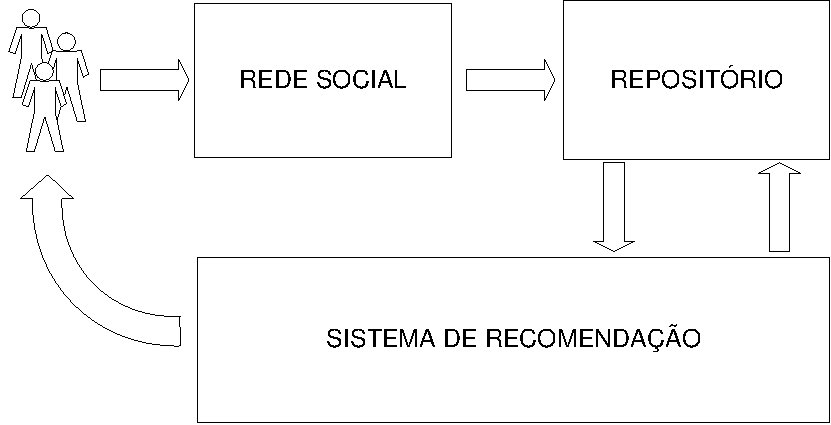
\includegraphics[width=\textwidth]{imagens/Diagrama_Visao_Geral}
  \caption{\it Diagrama de blocos do sistema}
  \label{fig:escopo}
\end{figure}

A Figura~\ref{fig:escopo} exibe o diagrama de blocos do sistema.


\section{Funcionalidades principais} % (fold)
\label{sec:funcionalidades_principais}

Abaixo estão sumarizadas as principais funcionalidades do sistema:

\begin{itemize}

	\item Recomendação de produtos baseada em preferência do usuário
	\subitem Como usuário, eu quero receber uma lista de produtos que eu provavelemente goste para que eu não precise filtrar os itens que me interessam.

	\item Permitir que o usuário avalie um produto
  \subitem Como usuário, quero fazer a minha avaliação de produtos para que outros tenham conhecimento da minha opinião.

	\item Permitir que o usuário envie uma recomendação a outro usuário
  \subitem Como recomendador, quero enviar uma recomendação de produto para outra pessoa para que ela conheça a minha opinião sobre este item.

	\item Exposição das avaliações em formatos abertos
  \subitem Como agente web, quero obter as avaliações dos usuários em formato padronizado (e aberto) para que possa interpretar estas avaliações.

    \item Inserção de novos produtos a partir de formatos abertos
    \subitem Como usuário, quero poder inserir em formato aberto um novo produto que ainda não está cadastrado.

    \item Explicação automática ao usuário do porquê daquele item ter sido recomendado
    \subitem Como usuário, quero saber porque aquele produto me foi recomendado.

    \item Visualização das avaliações dos amigos
    \subitem Como usuário, quero estar ciente sobre como meus amigos avaliaram produtos (para que eu possa conhecer novos produtos)

    \item Feedback de recomendação
    \subitem Como recomendador, quero receber feedback sobre as recomendações que enviei para poder fazer melhores recomendações.

	
\end{itemize}

\section{Requisitos não-funcionais}

Os principais requisitos não-funcionais do sistema são:

\begin{itemize}

    \item Interface web compatível as últimas versões dos \textit{browsers} Internet Explorer, Mozilla Firefox e Safari.
    
    \item \textit{Backend} compatível com servidores Linux.

    \item Tempo médio de resposta menor que 2 segundos para 10 usuários simultâneos quando executado em um servidor com processador Intel Core 2 Duo T7250 ou superior e 2 GB de memória RAM. % esta é a configuração do meu notebook -- Allan

\end{itemize}

\section{Limites do Sistema}

\begin{itemize}
    \item O sistema não fará processamento de linguagem natural\footnote{\textit{Natural Language Processing (NLP)}}

\end{itemize}

\section{Tecnologia} % (fold)
\label{sec:tecnologia}

% section tecnologia (end)

\section{Planejamento e Métodos} % (fold)
\label{sec:planejamento_e_métodos}


% section planejamento_e_métodos (end)

% chapter especificacao_do_projeto (end)

\chapter{TESTES} % (fold)
\label{cha:testes} % (fold)

\section{Descrição do Experimento}
\label{cha:descricao_do_experimento}

 Será feito um experimento para teste do Sistema de Recomendação de Produtos Dionisio.

 Dionisio é um Sistema que armazena informações sobre produtos e pessoas. As pessoas podem formar uma rede social de amigos e avaliar os produtos, fazendo recomendações para outras pessoas conhecidas ou desconhecidas. A partir das avaliações das pessoas e das relações sociais, o sistema gera listas de recomendações de produtos com o objetivo de ajudar as pessoas a encontrar produtos que elas ainda não conhecem mas possuem grande probabilidade de gostar.

 O experimento consistirá de um período de uso do sistema por grupos de pessoas. Serão 12 grupos com 5 pessoas cada um. Os grupos serão formados da seguinte forma:

\begin{itemize}
	\item Inicialmente serão convidadas 12 pessoas de diferentes faixas etárias.
	\item Será passado um endereço de internet (URL) para cada uma das pessoas se cadastrar no sistema
	\item Será pedido a cada uma dessas pessoas que convide mais 4 amigos ou conhecidos, usando uma ferramenta do próprio sistema, para completar um grupo de 5 pessoas.
\end{itemize}

 O cadastro no sistema consiste de um série de formulários que visam extrair informações demográficas e pessoais. Serão pedidas as seguintes informações:
 
\begin{itemize}
	\item Nome
	\item Sexo (masculino ou feminino)
	\item Data de nascimento
	\item Escolaridade
	\item Foto
\end{itemize}

 Será pedido também que elas avaliem em uma escala de 1 a 10, quais são os produtos que elas possuem o maior interesse para obter recomendações, como:

\begin{itemize}
	\item Roupas
	\item Músicas
	\item Filmes
	\item Eletrônicos
	\item Livros
\end{itemize}

	Depois do cadastro dessas informações iniciais será pedido que cada pessoe avalie as outras pessoas de seu grupo, fornecendo as seguintes informações sobre a outra pessoa:

\begin{itemize}
	\item O quanto ela conhece a outra pessoa. As opções são:
	\subitem Não conhece
  \subitem Conhece pouco
  \subitem Conhece bastante
  \subitem Melhor amiga
  \item O quanto ela confia na outra pessoa para a recomendação de produtos em geral:
  \subitem Não confia
	\subitem Confia um pouco
  \subitem Confia muito
  \subitem Confia completamente
\end{itemize}

 Após o levantamento dessas informações será pedido que cada usuário avalie uma série de produtos aleatórios. Cada produto será apresentado através de uma foto e uma descrição. Será pedido que o usuário escolha em uma escala de 1 a 5 o quanto ele gosta daquele produto caso ele o conheça. Se o usuário não conhecer o produto ele deverá escolher a opção "não conheço".

 Feita essa avaliação, começará o uso pleno do sistema pelo usuário. Dentro do sistema as pessoas terão as seguintes opções:
\begin{enumerate}
	\item Ver listas de recomendações
	\item Procurar por produtos
	\item Fazer uma recomendação
	\item Ver lista de pessoas
\end{enumerate}

 Ao acionar a primeira opção será mostrado ao usuário uma série de diferentes listagens de produtos recomendados. Para cada produto recomendado, o usuário terá a opção de avaliar:

\begin{itemize}
	\item O quanto ele gostou daquela recomendação, em uma escala de 1 a 5.
	\item Opcionalmente, o quanto ele gosta daquele produto.
\end{itemize}

 Uma destas listagens será composta pelas recomendações feitas por outras pessoas. Neste caso também será mostrado além do produto recomendado, quem fez a recomendação e uma justificativa do recomendado para aquela recomendação.

 Ao acionar a segunda opção, o usuário poderá ver os diferentes produtos cadastrados no sistema, podendo filtrá-los através de diferentes critérios. Haverá também uma listagem ordenada dos produtos mais bem avaliados nas diferentes categorias de produtos.

 Ao acionar a terceira opção, o usuário poderá fazer uma busca de um produto para recomendar a uma ou mais pessoas cadastradas no sistema. A recomendação consistirá de um produto e de uma justificativa do porquê daquele produto estar sendo recomendado.

 Ao acionar a quarta opção o usuário poderá ver a lista das pessoas conhecidas ou desconhecidas. Inicialmente apenas as pessoas de seu grupo estarão na lista de conhecidos. Mas ele poderá escolher uma outra pessoa para entrar em sua lista de conhecidos fazendo um pedido de amizade.

 A lista de pessoas possui um atalho para o perfil de cada usuário. Este perfil é composto do nome, idade, sexo, foto da pessoa e uma lista dos produtos avaliados por essa pessoa.

 O sistema estará disponível por um período de 1 mês, sendo que ao final o mesmo será desativado e sua base de dados será analisada de forma anônima para se medir qual foi a eficácia das recomendações feitas pelo sistema e entre os usuários.

 \section{Protótipo}
 \label{cha:prototipo}

 Um protótipo do sistema foi desenvolvido para que se pudesse ter noção da usabilidade e do funcionamento do sistema de recomendação. Inicialmente as recomendações são realizadas sem levar em conta os dados de confiança e reputação entre usuários. A Figura~\ref{fig:tela_inicial_prototipo} mostra a página inicial do protótipo, contendo a listagem dos primeiros produtos presentes na base de dados e a opção do usuário fazer o \textit{login} no sistema.
 
\begin{figure}
  \centering
  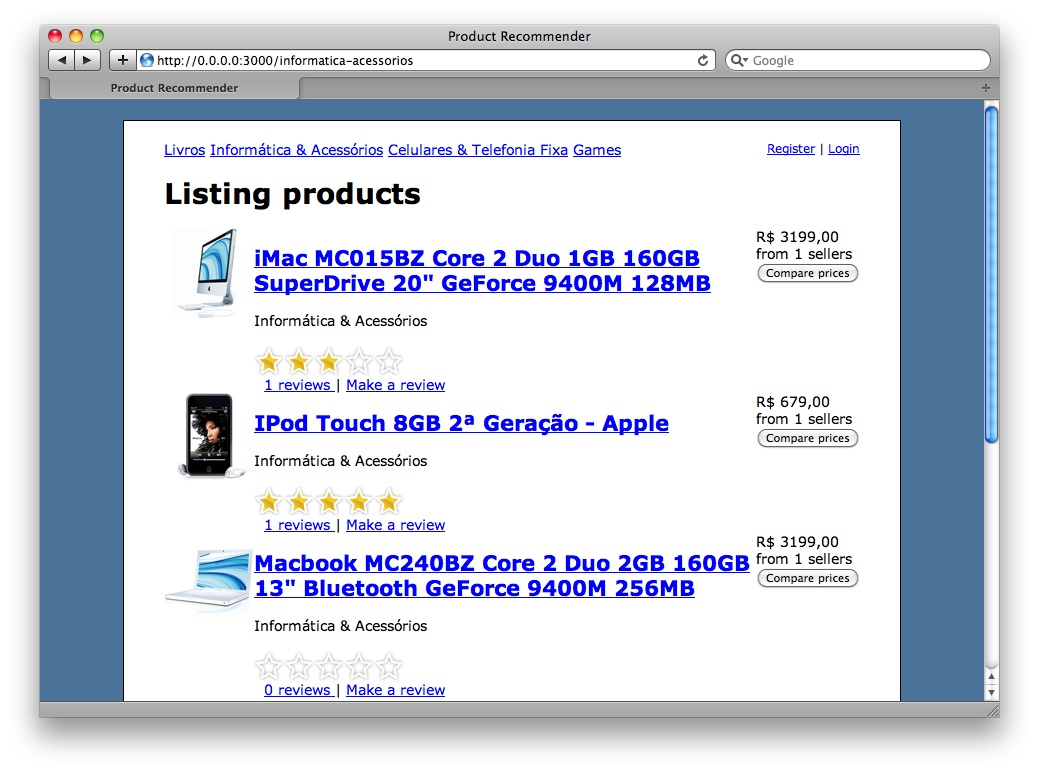
\includegraphics[width=\textwidth]{imagens/Tela_Inicial_Prototipo}
  \caption{\it Tela inicial do protótipo}
  \label{fig:tela_inicial_prototipo}
\end{figure}

 Para se cadastrar, a pessoa necessita apenas informar o seu nome de usuário, e-mail e entrar com uma senha pessoal. A tela de \textit{login} solicita apenas o nome de usuário e senha, conforme ilustrado na Figura~\ref{fig:tela_login_prototipo}. Após a validação dos dados, o sistema retorna para a tela inicial para que o usuário possa detalhar um produto de seu interesse. Há a opção de avaliar o produto sem conferir os seus detalhes. Para avaliar o produto o usuário escolhe de 1 a 5, sendo 1 não gostar do produto e 5 gostar muito, e clicar em uma das cinco estrelas. O número de estrelas coloridas mostra a nota da avaliação. 
 
 Para efetuar o \emph{login} o sistema solicita apenas o nome de usuário e senha. Após a autenticação, o sistema retorna para a tela inicial para que o usuário possa procurar um produto de seu interesse. Ao escolher um produto, o sistema abre os seus detalhes incluindo nome, foto e descrição completa, como mostra a Figura~\ref{fig:detalhe_produto_prototipo}.

\begin{figure}
  \centering
  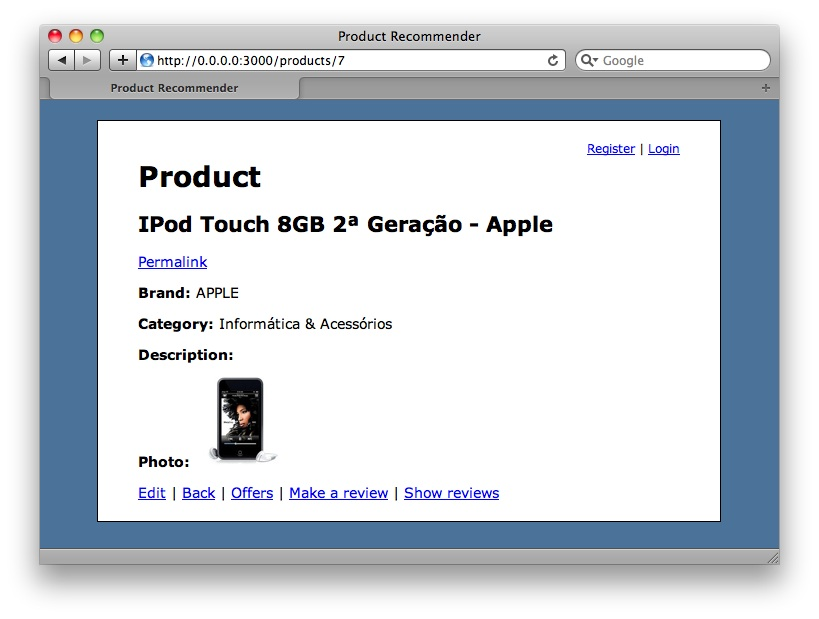
\includegraphics[width=\textwidth]{imagens/Detalhe_Produto_Prototipo}
  \caption{\it Detalhe do produto}
  \label{fig:detalhe_produto_prototipo}
\end{figure}

 Na tela de detalhamento do produto o usuário poderá editar as informações do mesmo ao escolher a opção \textit{edit}. Também é possível visualizar os comentários (\textit{reviews}) feitos pelos usuários sobre o produto detalhado, além de fazer o seu próprio comentário, clicando em \textit{Make a review}.
  
 A encontrar um produto interessante o usuário tem a opção de recomendá-lo para outros da rede social. A opção \emph{Recommend it!} leva o usuário a tela ilustrada na Figura~\ref{fig:recomendacao_produto_prototipo}, onde é possível selecionar os amigos para os quais a recomendação será enviada.

 \begin{figure}
   \centering
   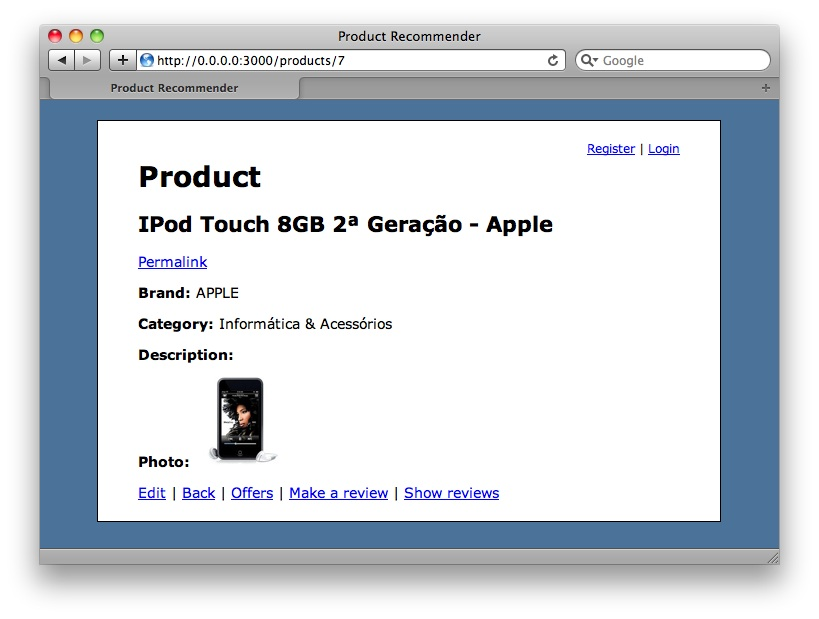
\includegraphics[width=\textwidth]{imagens/Detalhe_Produto_Prototipo}
   \caption{\it Detalhe do produto}
   \label{fig:detalhe_produto_prototipo}
 \end{figure}         
 
 \begin{figure}
   \centering
   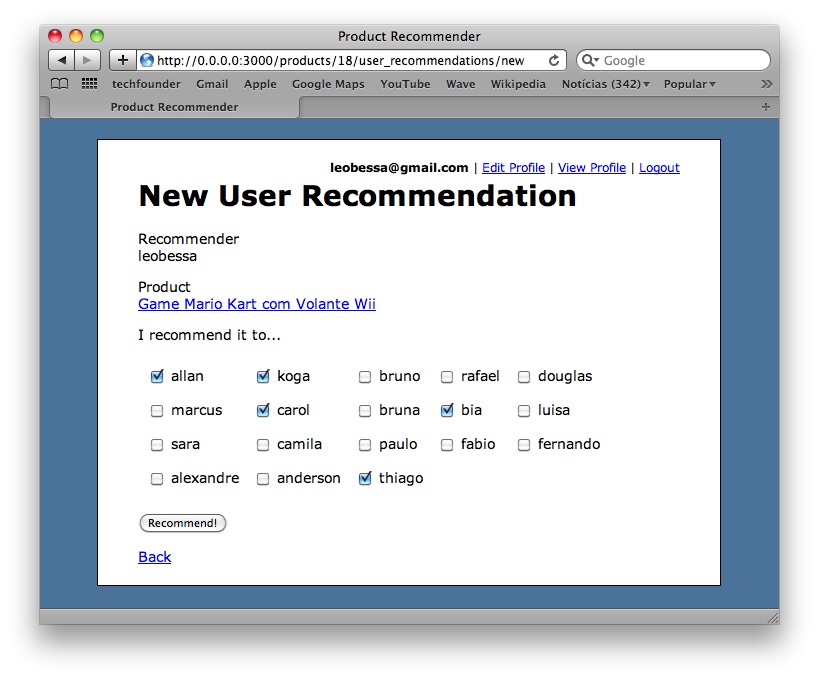
\includegraphics[width=\textwidth]{imagens/TELA_RECOMENDACAO_PROTOTIPO}
   \caption{\it Tela de recomendação de produto}
   \label{fig:recomendacao_produto_prototipo}
 \end{figure}

%\include{capitulos/5-metodologia}
%\include{capitulos/6-implementacao}
%\include{capitulos/8-conclusoes}

\addcontentsline{toc}{chapter}{Referências Bibliográficas}
\bibliographystyle{abnt-num}   %\bibliographystyle{plain}
\bibliography{capitulos/bibliografia} % bibname=nome do seu arquivo BibTeX
\begin{thebibliography}{99}

 

%  \bibitem{marketing_social_web}
%    WEBER, LARRY.
%    \textbf{Marketing to the social web}: how digital customer communities build your business.
%    Wiley, 2007, 5 p.

\end{thebibliography}


%\addcontentsline{toc}{chapter}{Glossário}
%\chapter*{Glossário} % (fold)
\label{cha:glossario}

\begin{itemize}

  \item \emph{ADSL}: acrônimo de \emph{Asymmetric Digital Subscriber Line}, é uma forma de transmissão de dados de alta velocidade utilizando linhas telefônicas comuns, em freqüências maiores que os seres humanos conseguem escutar.

  \item \emph{BNC}: é um tipo de conector cujo nome vem de seus criadores: ``bayonet Neil-Concelman''. Sua grande característica é o sistema de trava, tipo twist-lock (gira e trava), que possibilita grande segurança na conexão. É bastante utilizado nos equipamentos profissionais de vídeo.

  \item \emph{Broadcast}: é um modo de difusão de sinais em que é transmitido o mesmo conteúdo para todos os receptores. Numa transmissão de TV, por exemplo, todas as pessoas sintonizadas no mesmo canal assistem ao mesmo programa. Em Internet, o termo é usado muitas vezes para designar o envio de uma mensagem par todos os membros de um grupo, em vez da remessa para membros específicos.

  \item \emph{Buffer}: é uma área de armazenamento que compensa diferentes velocidades de fluxos de dados ou temporizações de eventos, ao transferir dados de um dispositivo para outro.

  \item \emph{CD}: acrônimo de Compact Disc, é um padrão de armazenamento óptico para dados digitais.
  Conversor A/D: um Conversor Analógico-Digital é componente de um sistema responsável por converter dados analógicos para digitais através da amostragem de um sinal contínuo e sua posterior discretização gerando valores numéricos digitais.

  \item \emph{Classpath}: é um argumento passado para a Java Virtual Machine indicando onde procurar classes e pacotes para carregamento dinâmico.

  \item \emph{CPqD}: {C}entro de {P}es{q}uisa e {D}esenvolvimento em Telecomunicações.

  \item \emph{DivX}: é um formato de compactação de vídeo criado pela DivxNetworks Inc.

  \item \emph{Driver}: um driver é um componente de software responsável por estabelecer a comunicação entre hardware e software, provendo comandos para enviar e receber dados de um dispositivo instalado.

  \item \emph{DVD}: acrônimo de Digital Versatile Disc, é a geração seguinte ao CD, possibilitando um armazenamento maior de dados.

  \item \emph{ECMAScript}: é uma linguagem de programação baseada em scripts, padronizada pela Ecma International na especificação ECMA-262. A linguagem é bastante usada em tecnologias para Internet, sendo esta base para a criação do JavaScript/JScript e também do ActionScript.

  \item \emph{FIFO}: acrônimo para {F}irst {I}n, {F}irst {O}ut (que em português significa primeiro a entrar, primeiro a sair) refere-se a estruturas de dados do tipo fila onde os elementos vão sendo colocados e retirados (ou processados) por ordem de chegada.

  \item \emph{GEM}: acrônimo de \emph{Globally Executable MHP} \cite{gem}, é uma parte do MHP independente dos padrões de transmissão europeus, criado com a finalidade de padronizar partes de todos os padrões de \emph{middleware} mundiais e possibilitar a criação de aplicações que funcionem em qualquer \emph{middleware} que seja compatível com o GEM.

  \item \emph{GSM}: acrônimo de Global System for Mobile Communications é um dos principais padrões para telefonia móvel existente.

  \item \emph{Heap}: Heap de objetos é o nome dado a parte da memória do computador que contém a estrutura de dados responsável por armazenar todos os objetos durante a execução da máquina virtual Java.

  \item \emph{HTTP}: acrônimo para {H}yperText {T}ransfer {P}rotocol (Protocolo de Transferência de Hipertexto), utilizado para transferência de dados na rede mundial de computadores, a World Wide Web.

  \item \emph{IPC (Inter-Process Communication)}: é o grupo de mecanismos que permite aos processos transferirem informação entre si. Entre estes mecanismos podem ser citados pipes, filas de mensagens e memória compartilhada.

  \item \emph{Java}: é uma linguagem de programação orientada a objeto desenvolvida na década de 90 pelo programador James Gosling, na empresa Sun Microsystems.

  \item \emph{JavaBeans}: são componentes reutilizáveis de software escritos em linguagem Java, e que seguem algumas convenções de modo a permitir que ferramentas possam utilizá-los e manipulá-los.

  \item \emph{JavaTV}: é uma biblioteca Java que contempla a maior parte dos recursos necessários para a operação de sistemas receptores de TV digital, simplificando assim o desenvolvimento de softwares, uma vez que os programadores de aplicativos podem se voltar ao tema principal da aplicação em desenvolvimento.

  \item \emph{JNI (Java Native Interface)}: é um padrão de programação que permite que a máquina virtual da linguagem Java acesse bibliotecas construídas com o código nativo de um sistema.

  \item \emph{Lista ligada}: é uma estrutura de dados linear e dinâmica composta por células que apontam para o próximo elemento da lista.

  \item \emph{Metodologia (Processo) de Desenvolvimento Ágil}: metodologias de desenvolvimento ágil foram pensadas de forma a minimizar riscos no desenvolvimento de software através períodos mais curtos de lançamento, chamados iterações, que tipicamente levam de uma quatro semanas. Métodos ágeis prezam mais a comunicação face-a-face que a documentação, como forma de acelerar o processo de desenvolvimento.

  \item \emph{MHP}: acrônimo de \emph{Multimedia Home Platform} \cite{mhp}, é um padrão aberto de \emph{middleware} para TV Digital, adotado principalmente pelos países europeus. Está incluso em outro padrão maior, o \emph{Digital Video Broadcasting} (DVB) \cite{dvb} que agrupa todas as características da tecnologia de TV Digital européia.

  \item \emph{Middleware} (conforme \cite{ginga}): é a camada de software intermediário que permite o desenvolvimento de aplicações interativas para a TV Digital de forma independente da plataforma de hardware dos fabricantes de terminais de acesso (\emph{set-top boxes}).

  \item \emph{MPEG}: acrônimo para {M}oving {P}icture {E}xperts {G}roup, é o grupo de trabalho da Organização Internacional para Padronização (ISO) para o desenvolvimento de padrões para vídeo e áudio digitais.

  \item \emph{MPEG2}: é um padrão de compressão e codificação de vídeo para difusão e comunicações, bem como para armazenamento em meios diversos, tais quais os ópticos.

  \item \emph{MPEG-TS}: MPEG {T}ransport {S}tream (TS, TP, ou MPEG-TS) é um protocolo de  comunicação para transmissão de áudio, vídeo e dados, especificado pelo padrão  ISO/IEC 13818-1. Permite multiplexar vídeo e áudio digital sincronizando a saída. Possui correção de erro e transporte, e é usado para difusão de aplicações como DVB e ATSC.

  \item \emph{MOV}: formato de vídeo criado pela Apple, é um container para imagem, diversas trilhas, efeitos e textos. Sua base foi aprovada pela ISO como padrão para MPEG4 Part. 14.

  \item \emph{Multiplexação no tempo}: a multiplexação no tempo consiste na transmissão de dois ou mais sinais ou fontes de bits simultaneamente através de um único canal pela divisão do tempo em pequenos compartimentos de tamanhos fixos, onde são transmitidos alternadamente um pouco de cada sinal.

  \item \emph{Overhead}: Em computação overhead é geralmente considerado qualquer processamento ou armazenamento em excesso, seja de tempo de computação, de memória, de largura de banda ou qualquer outro recurso que seja requerido para ser utilizado ou gasto para executar uma determinada tarefa.

  \item \emph{Pipe (UNIX)}: é o redirecionamento da saída padrão de um programa para a entrada padrão de outro.

  \item \emph{{S}et-{t}op {B}ox ({STB})}: é o termo que descreve um equipamento que se conecta a um televisor e a uma fonte externa de sinal, transformando este sinal em conteúdo no formato que possa ser apresentado em uma tela.

  \item \emph{SBTVD} \cite{sbtvd}: acrônimo para {S}istema {B}rasileiro de {TV} {D}igital.

  \item \emph{SMS}: acrônimo para {S}hort {M}essage {S}ervice. Tecnologia amplamente utilizada em telefonia celular para a transmissão de mensagens de texto curtas.

  \item \emph{SOAP}: acrônimo de \emph{Service Oriented Architecture Protocol}, é um protocolo de troca de mensagens em formato XML.

  \item \emph{Thread}: é uma forma de um processo dividir a si mesmo em duas ou mais tarefas que podem ser executadas simultaneamente.

  \item \emph{UML}: acrônimo de Unified Modelling Language, é um padrão gráfico de especificação para modelagem de objetos, e uma ferramenta importante no processo de desenvolvimento de software.

  \item \emph{{USB}}: acrônimo de {U}niversal {S}erial {B}us, é uma especificação para interfaces de comunicação serial de dados. É padronizado pelo {USB} {I}mplementers {F}orum ({USB-IF}), que possui membros como Apple Inc., Hewlett-Packard, NEC, Microsoft e Intel.

  \item \emph{W3C}: acrônimo de World Wide Web Consortium, é o principal órgão de padronização para a Web (Internet).

  \item \emph{Web Services}: é definido pelo W3C como um sistema de software projetado para dar suporte à comunicação interoperável entre duas máquinas utilizando uma rede. Essa comunicação é feita através de mensagens XML utilizando-se servidores web, em um padrão denominado SOAP.

  \item \emph{Wi-Fi}: é uma marca registrada pertencente à Wireless Ethernet Compatibility Alliance (WECA), e é a abreviatura de \emph{wireless fidelity}, sendo uma tecnologia de interconexão entre dispositivos sem fio, usando o protocolo IEEE 802.11.

  \item \emph{WiMax}: acrônimo de \emph{Worldwide Interoperability for Microwave Access}, é o nome comercial para o padrão IEEE 802.16, que especifica uma interface sem fio para redes metropolitanas, agregando conhecimentos e recursos mais recentes ao padrão Wi-Fi visando melhor performance de comunicação.

  \item \emph{WMV}: \emph{Windows Media Video} é o nome para uma série de formatos de vídeo compactados criados pela Microsoft.

  \item \emph{XHTML}: acrônimo para \emph{eXtensible HyperText Markup Language}, é uma linguagem de marcação com as mesmas marcas do HTML, porém com uma sintaxe mais rigorosa pois é baseada no XML, e dessa podem ser validadas com bibliotecas XML.

  \item \emph{XML}: acrônimo para \emph{eXtensible Markup Language}, é uma especificação para uma linguagem de marcação de uso geral, permitindo que possam ser criados novas linguagens.

  \item \emph{XviD}: formato de compactação de vídeo competidor direto do DivX. Enquanto o DivX é um formato proprietário, o XVid é livre e de código aberto, disponível para diferentes plataformas.

  \item \emph{YouTube}: é um site na Internet que permite que seus usuários carreguem, assistam e compartilhem vídeos em formato digital. Foi fundado em fevereiro de 2005 por três pioneiros do PayPal, um famoso site da internet ligado a gerenciamento de doações. Foi comprada em 9 de Outubro de 2006 pelo Google, pela quantia de US\$1,65 bilhões em ações.

\end{itemize}
% chapter glossário (end)



% anexos (opcional)
%\addcontentsline{toc}{chapter}{\appendixname}
%\appendix
%

%


% indice remissivo (opcional)

\end{document}
